% Chapter 1

\chapter{Automatic Metadata Extraction} % Main chapter title

\label{Chapter3} % For referencing the chapter elsewhere, use \ref{Chapter1} 

\lhead{Chapter 3. \emph{Automatic Metadata Extraction}} % This is for the header on each page - perhaps a shortened title

%----------------------------------------------------------------------------------------

\emph{In this chapter we define the problem of automatic metadata extraction, providing illustrations of the problem, its complexities, and discuss the methods by which the problem may be solved. Moreover, we introduce GROBID, the metadata extraction tool around which our work is based, and describe the cascade of CRF models it uses to solve the problem. Notably, we provide a comparison between GROBID and the existing solution for metadata extraction at CERN, REFEXTRACT.}

\section{Metadata Extraction}

Automatic metadata extraction (AME) has been referred to as `one of the hardest problems in document engineering'. In our work we are concerned with extraction for scientific articles that are usually (though not necessarily) in the form of a PDF document, as these predominate in the INSPIRE-HEP digital library. Nevertheless, the same techniques will be effective for books, theses, or may even have novel applications\footnote{Such as for segmenting cooking recipes, as reported in The New York Times (http://open.blogs.nytimes.com/2015/04/09/extracting-structured-data-from-recipes-using-conditional-random-fields/?\_r=0).}. At CERN, the problem has been partially solved, albeit in a rudimentary way, and also entails a lot of manual curation to complete the work. See Section \ref{subsec:refextract} for a comparison between this existing solution and GROBID, the leading tool for metadata extraction.

\emph{Metadata} refers to various information explicitly or implicitly contained in a scientific article. Perhaps the most important metadata for an article is that contained in the header, that is, the text at the front of a document, typically containing the title of the article as well as the names, affilations and often the contact details of the authors, concluding finally with the article abstract. As a general rule, this is tantamount to the text of the document falling before the first section of the body (usually called `Introduction'), though as we find in Chapter \ref{Chapter4}, sometimes significant amounts of front matter is held in unexpected places. Other important types of metadata may be the references of the article, typically classified into fields such as publication title, authors, data of publication, and so on. Another potential metadata type is that of the document structure, its chapters and sections. All of these types are modelled by GROBID.

\emph{Extraction} could refer to either of two distinct concepts. First, it may be the parsing of a PDF document and extraction of plaintext and images. This in itself is a complex problem, and may involve machine learning techniques for OCR analysis, depending on the rendering of the document. Or, it may be the \emph{classification} of document content into predefined categories. It is on the second idea that we are focused within this work. Indeed, GROBID addresses both of these points, but the first is merely a precondition for the analysis it is primarily concerned with, and it houses a third-party PDF to XML conversion tool, \emph{pdftoxml}, developed at Xerox Research Centre Europe (XRCE), to handle this (\cite{dejean2006system}).

To appreciate the difficulty of automating such a task, contrast Figures \ref{fig:header1} and \ref{fig:header2} in Appendix \ref{AppendixB}, contrasting the header sections of two articles from our dataset. Though the same sorts of information are present in both headers--title, author names, affiliations, and document abstract--the arrangement and presentation of these fields are different, for example the sizing and placement of the document title, the juxtapositioning of authors (which are in variable in number) and author details, and labelling of the abstract block. Furthermore, the second header is more complete, in that it contains information not present in the other, for example copyright and publication details. The contents of a document header do not follow a predictable sequencing, making the problem hard, but are not entirely random, a condition that would render the problem impossible to solve. There is structure to a document, but it is likely infeasible to model deterministically. Therefore, we must look to probabilistic approaches, and accept that these will be error-prone. Also, if we are to process an entire document, it is unlikely we can create a one-size-fits-all model, rather, the problem must be decomposed.

\begin{figure}[!ht]
\center
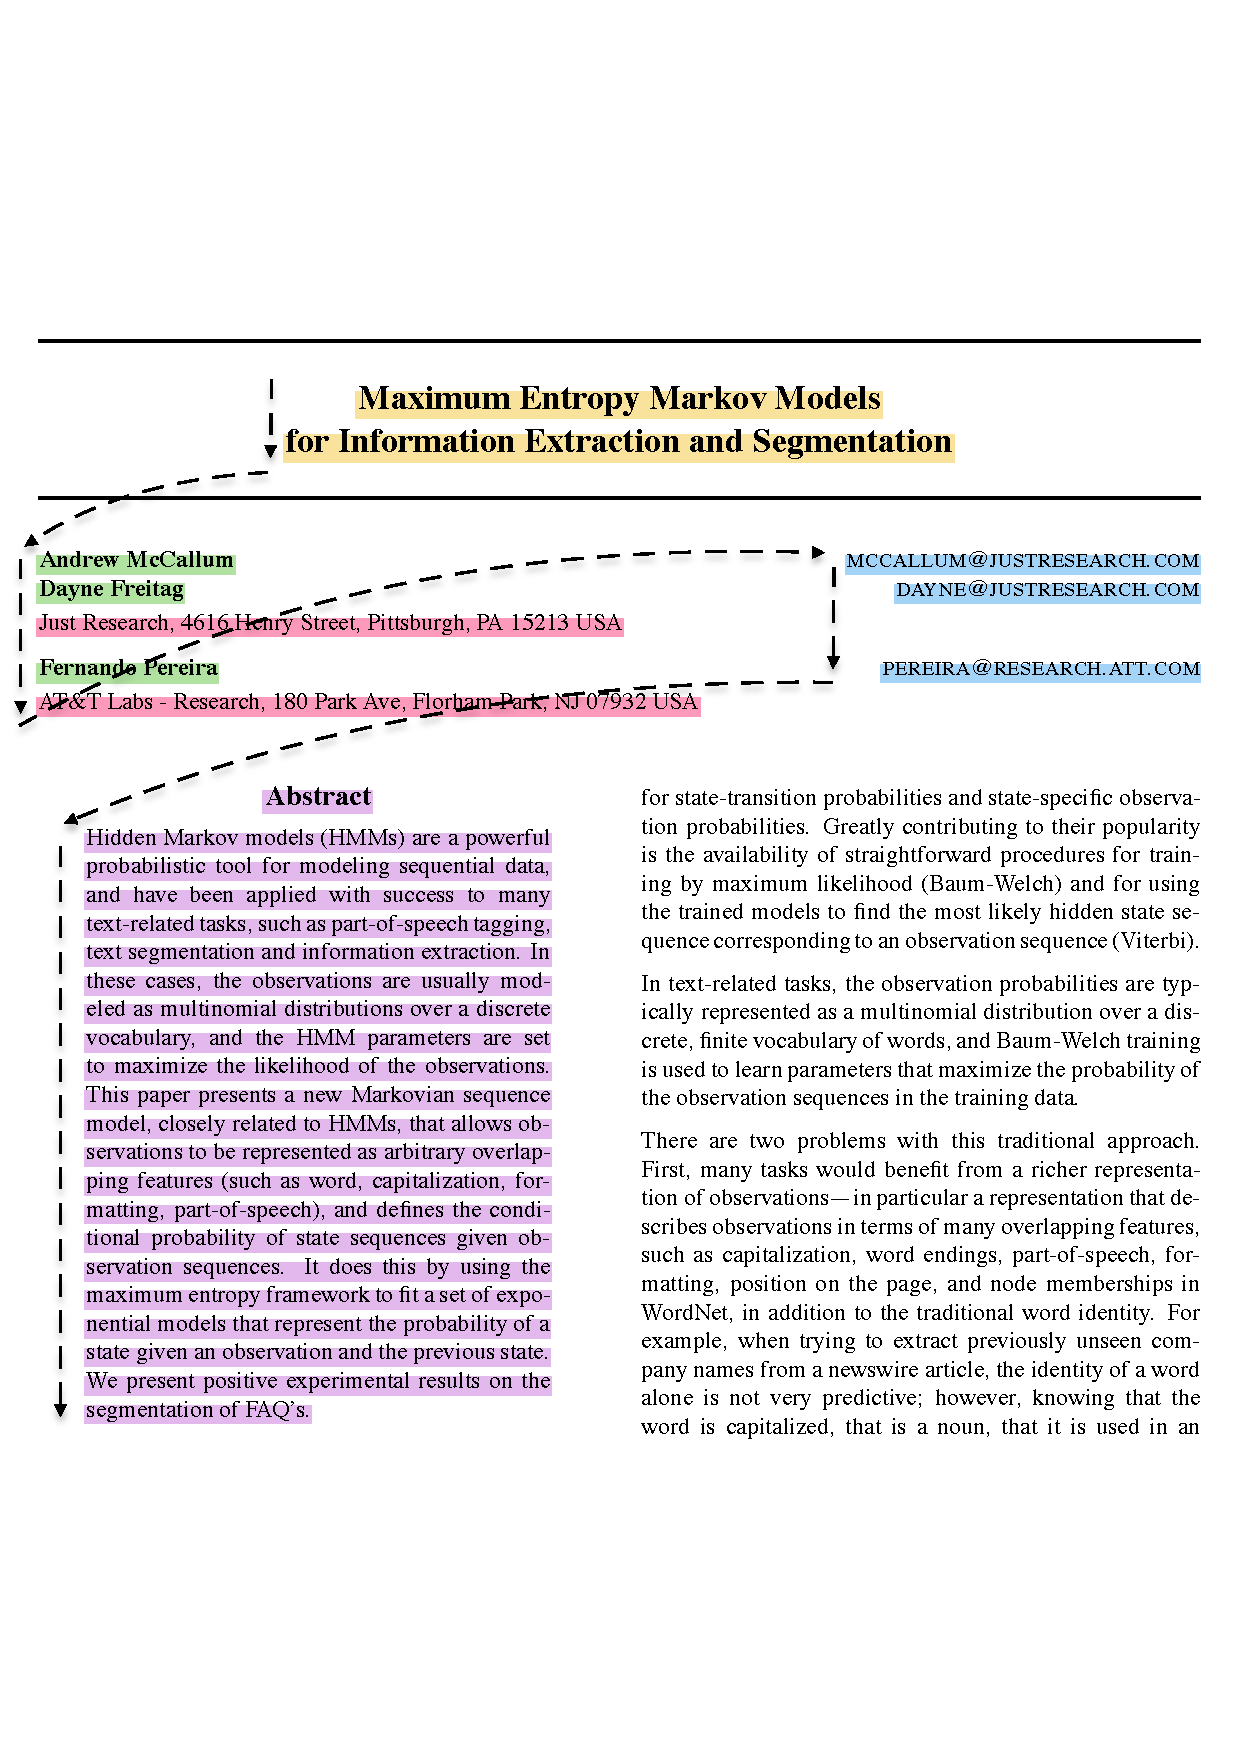
\includegraphics[width=\textwidth]{Figures/extraction.pdf}
\caption{An illustration of the way a header section might be segmented and classified. The classes modelled are colour-code (title in yellow, authors in green, and so on).}
\label{fig:grobid}
\end{figure}

\section{Solution Methods}

A 2013 study of metadata extraction techniques \cite{lipinski2013evaluation} identified three fundamental methods for AME:

\begin{enumerate}
\item stylistic analysis;
\item knowledge base, and;
\item machine learning approaches.
\end{enumerate}

\emph{Stylistic analysis} refers to heuristic approaches to analysing physical characteristics of text font and layout. \emph{Knowledge base} methods rely on online repositories to cross reference extracted information. \emph{Machine learning} refers here either to the state-of-the-art conditional random fields, or to other approaches such as hidden Markov models or support vector machines. There is evidence to suggest that the best approach is a combination of the three methods, and the study admits software systems such as GROBID (Section \ref{sec:grobid}) do so. The study includes a comparison of the leading AME tools based on an ad hoc scoring system over fixed header extraction test data. GROBID performed best by a considerable margin, ahead of commercial applications Mendeley Desktop and ParsCit.

\section{GROBID}
\label{sec:grobid}
GROBID (GeneRatiOn of BIbliographic Data) (\cite{lopez2009grobid}) is an open-source (Apache license) Java-based tool for automatic metadata extraction of scientific articles. It has been in development by Patrice Lopez at the French Institute for Research in Computer Science and Automation (INRIA) since 2008. Grobid manages the training, evaluation and application of a hierarchy of Wapiti-trained CRF models, each addressing a part of the information extraction of scientific articles. Figure \ref{fig:cascade} shows the \emph{cascade} of models used to progressively refine classifications of article content. Through GROBID, higher-tier models such as the \emph{header} and \emph{reference} models may be applied individually to PDFs, while the other, more specific models, such as the \emph{date} model, operate only on plaintext inputs. Moreover, some models such as \emph{segmentation} are not intended to be used independently, but rather contribute to the cascade, supplying lower levels with information. For example, reference extraction begins with segmentation models, which classify each line of a document, resulting in homogenous blocks of lines e.g. header, paragraph, figure, references. This information is then distributed to the other models, for example the \emph{reference segmenter} model, which further breaks down the reference list into individual references. The \emph{citation} model then classifies the parts of each reference into classes, for example, \emph{date}, \emph{affiliation}, and \emph{author}. Finally, the atomic subcomponents of these are classified by their respective models. Note that the \emph{citation} branch of the cascade has the option of further cross-checking extracted references with the third-party CrossRef web service\footnote{CrossRef is a online RESTful service.}. Thus, the overall accuracy of the system is dependent on the combined accuracy of models. Though they have much in common, the models vary in the classifications they assign, the features they exploit, and, due to the varying size of the vocabulary (compare say, the number of possible month names to the number of possible author names), the size (dimensionality) of the models. Table \ref{table:featurelist} summarises each of GROBID's models. Calling GROBID function \texttt{processFullText} runs all available models on a batch of PDF documents and classifies each document entirely.

Both training and evaluation are performed on sets of TEI documents (see Section \ref{subsec:tei}). This is also the output format for prediction, so there is consistency between input and output formats. It may appear paradoxical to \emph{evaluate} the tool on TEI files, rather than PDFs. However, with closer inspection of the source code, an equivalence can be seen between:

\begin{enumerate}
\item applying an OCR tool (pdftoxml), tokenising the output and transforming to CRF input data, and;
\item extracting tokens from TEI documents, and transforming to CRF input data.
\end{enumerate}

Both approaches yield the same input data for the CRF engine, and so evaluation is in fact equivalent to prediction, despite the initial difference in input formats. Figure \ref{fig:traininput} shows an excerpt from an input file to the CRF engine for training. The feature function templates (see Section \ref{subsec:featuretemplates}) for each model are contained in a separate file. It is therefore vital that the feature extraction, which is generated by Grobid, is aligned with the template file, which is manually configured by the developer. As depicted in Figure \ref{fig:flow}, there is a strong coupling between these two parts of Grobid.

\begin{center}
\begin{table}
\begin{tabular}{ | p{0.15\linewidth} | p{0.35\linewidth} | p{0.4\linewidth} |}
	\hline
	Model & Description & Labels \\ \hline
    Header & Classifies front matter & <title>, <author>, <affiliation>, <reference>, <submission>, <abstract>, <address>, <keyword>, <degree>, <pubnum>, <email>, <date>, <copyright>, <intro>, <web>, <note>, <phone>, <dedication>, <entitle>, <grant>, <date-submission> \\ \hline
	Affiliation address & Classifies the components of author affiliations and affiliation addresses. Subordinate to the \emph{header} model. & <institution>, <other>, <settlement>, <department>, <postcode>, <contry>, <marker>, <region>, <addrLine>, <laboratory>, <postbox>, <other>, <null> \\ \hline
	Name/ Header & Classifies an authors full name (as identified by the \emph{header} model) into first and last name components etc.  & <forname>, <surname>, <marker>, <middlename>, <other>, <suffix>, <title> \\ \hline
	Name/ Citation &  Classifies an authors full name (as identified by the \emph{citation} model) into first and last name components etc. & <surname>, <forname>, <other>, <middlename> \\ \hline
	Citation & Classifies a reference into its subcomponents. & <journal>, <volume>, <other>, <issue>, <pages>, <date>, <author>, <title>, <booktitle>, <location>, <pubnum>, <note>, <publisher>, <editor>, <institution>, <tech>, <web>, <issue> \\ \hline
	Date & Classifies the components of a date string identified by higher-tier models. & <other>, <day>, <month>, <year> \\ \hline
	Segmentation & The highest-level model in the architecture--primarily supplies the three models beneath it (header, fulltext and reference-segmenter). & <headnote>, <header>, <body>, <page>, <references>, <footnote>, <cover>, <acknowledgement>, <annex> \\ \hline
	Reference-Segmenter & Segments a full reference list into individual citations. & <label>, <reference>, <other> \\ \hline
	Fulltext & Classifies elements of article body. & <section>, <paragraph>, <citation\_marker>, <other>, <table\_marker>, <figure\_marker>, <figure\_head>, <trash>, <figDesc>, <equation>, <item> \\ \hline
\end{tabular}
\caption{A summary of the models coordinated by GROBID. We have here excluded the Patent, Entities, and E-book models as these are experimental models not currently used by Grobid.}
\label{table:featurelist}
\end{table}
\end{center}

\subsection{Text Encoding Initiative}
\label{subsec:tei}
One of GROBID's features is to transform Wapiti outputs into a standard output conforming to the Text Encoding Initiative (TEI) standard, therefore we briefly describe it here. TEI is a text encoding standard maintained by the TEI consotrium. It specifies an XML representation of a document contents from the front matter, to the document body, to the document rear. It gives structure and semantic meaning to docment components, with little restriction to the level of detail desired. It is therefore apt as a iel format for annotating a document's metadata. GROBID uses TEI to format its outputs, as well as its training data. In Figure \ref{fig:tei}, we show a sample of a TEI document used to represent a date. The stuctured XML format can be used to give semantic information about the information enclosed. There is thus a natural mapping between metadata classification and the TEI schema.

\begin{figure}
\lstset{language=XML}
\begin{lstlisting}
<bibl>
    <author>V. Gundelach and D. Eisenburger</author>, &quot; 
    <title level="a">Principle of a direction sensitive borehole antenna with advanced technology and data examples</title>, &quot; in 
    <title level="m">Proceedings of the 4th International Workshop on Advanced Ground Penetrating Radar (IWAGPR &apos;07)</title>, pp. 
    <biblScope type="pp">28-31</biblScope>, 
    <date>June 2007</date>.
</bibl>
\end{lstlisting}
\caption{Sample tagged citation for Grobid training input.}
\label{fig:tei}
\end{figure}

\subsection{Evaluation}

Training may be done with a split defined by the developer, which Grobid will use to set aside a proportion of the training data for evaluation. The evaluation of a model produced by training follows identical procedures, preparing the same input data. The output, however, is not a model but a the input data with labels. Grobid compares its predictions with the ground truth and outputs \emph{precision}, \emph{accuracy} and \emph{F1 scores} as performance indicators, at the token, field, and instance levels. A token refers to a single contiguous string of characters (without spaces), a field is a block of contiguous tokens, and an instance is an entire document. Accuracy of an instance is therefore judged by the correctness of all tagging for the whole document, a difficult thing to achieve without any mistakes.

\subsection{Prediction}

Figure \ref{fig:flow} shows the flow of information from input to output, as well as the relationship between training and prediction. When it comes to labelling (prediction), the starting point is a PDF document. With a third-party tool, pdftoxml, this is transformed into an XML file containing OCR information (font, style, orientation) for every token in the document. This information is stored in LayoutToken objects within Grobid. These tokens are arranged into blocks and features are extracted as they were for training and evaluation. Excepting the absence of tokens, the input is the same. The model created in the training phase is first loaded, and then the EngineTagger calls the CRF engine to label the inputs. Unlike for training, the feature template file is not required, as these have already been absorbed into the model file. After processing, Wapiti returns the same file with tags inserted. Grobid then further processes this information to transform it into the final TEI format.

\subsection{Other Functionality}

In addition to the above, Grobid provides a means of producing training sets semi-automatically. This consists of applying the existing models on the training set to produce the XML inputs. Of course, each field must be checked against a ground truth and errors corrected before it is used as a training set. We intend to use this functionality to generate training data for benchmarking Grobid on HEP papers.

\begin{figure}[!ht]
\center
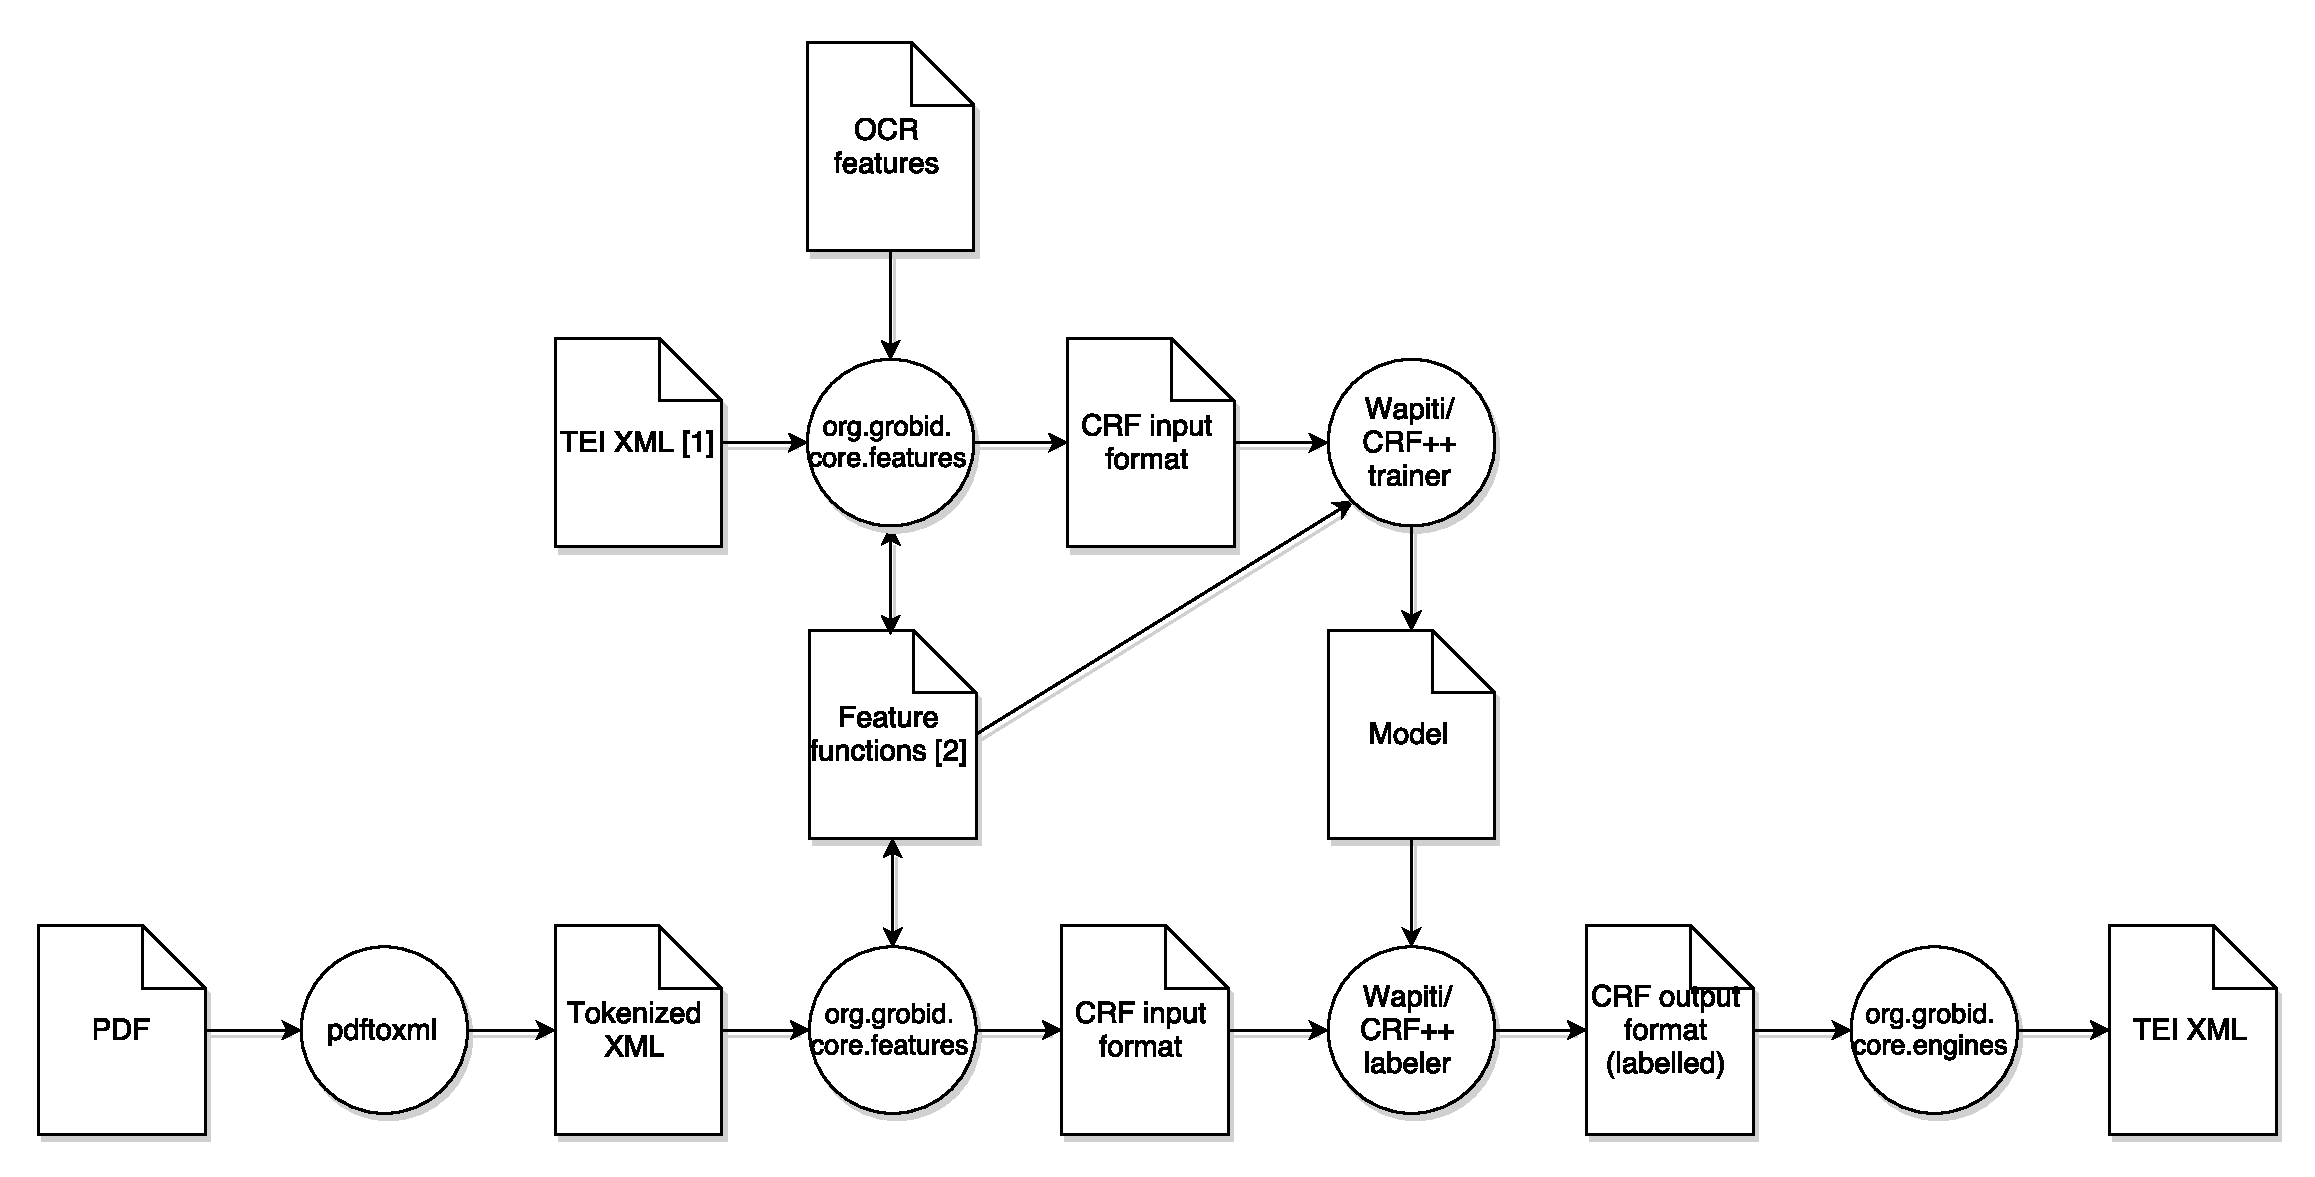
\includegraphics[width=\textwidth]{Figures/grobid.pdf}
\caption{An illustration of the interactions between Grobid and Wapiti for the two main functions of training and tagging.}
\label{fig:grobid}
\end{figure}

\begin{figure}[!ht]
\center
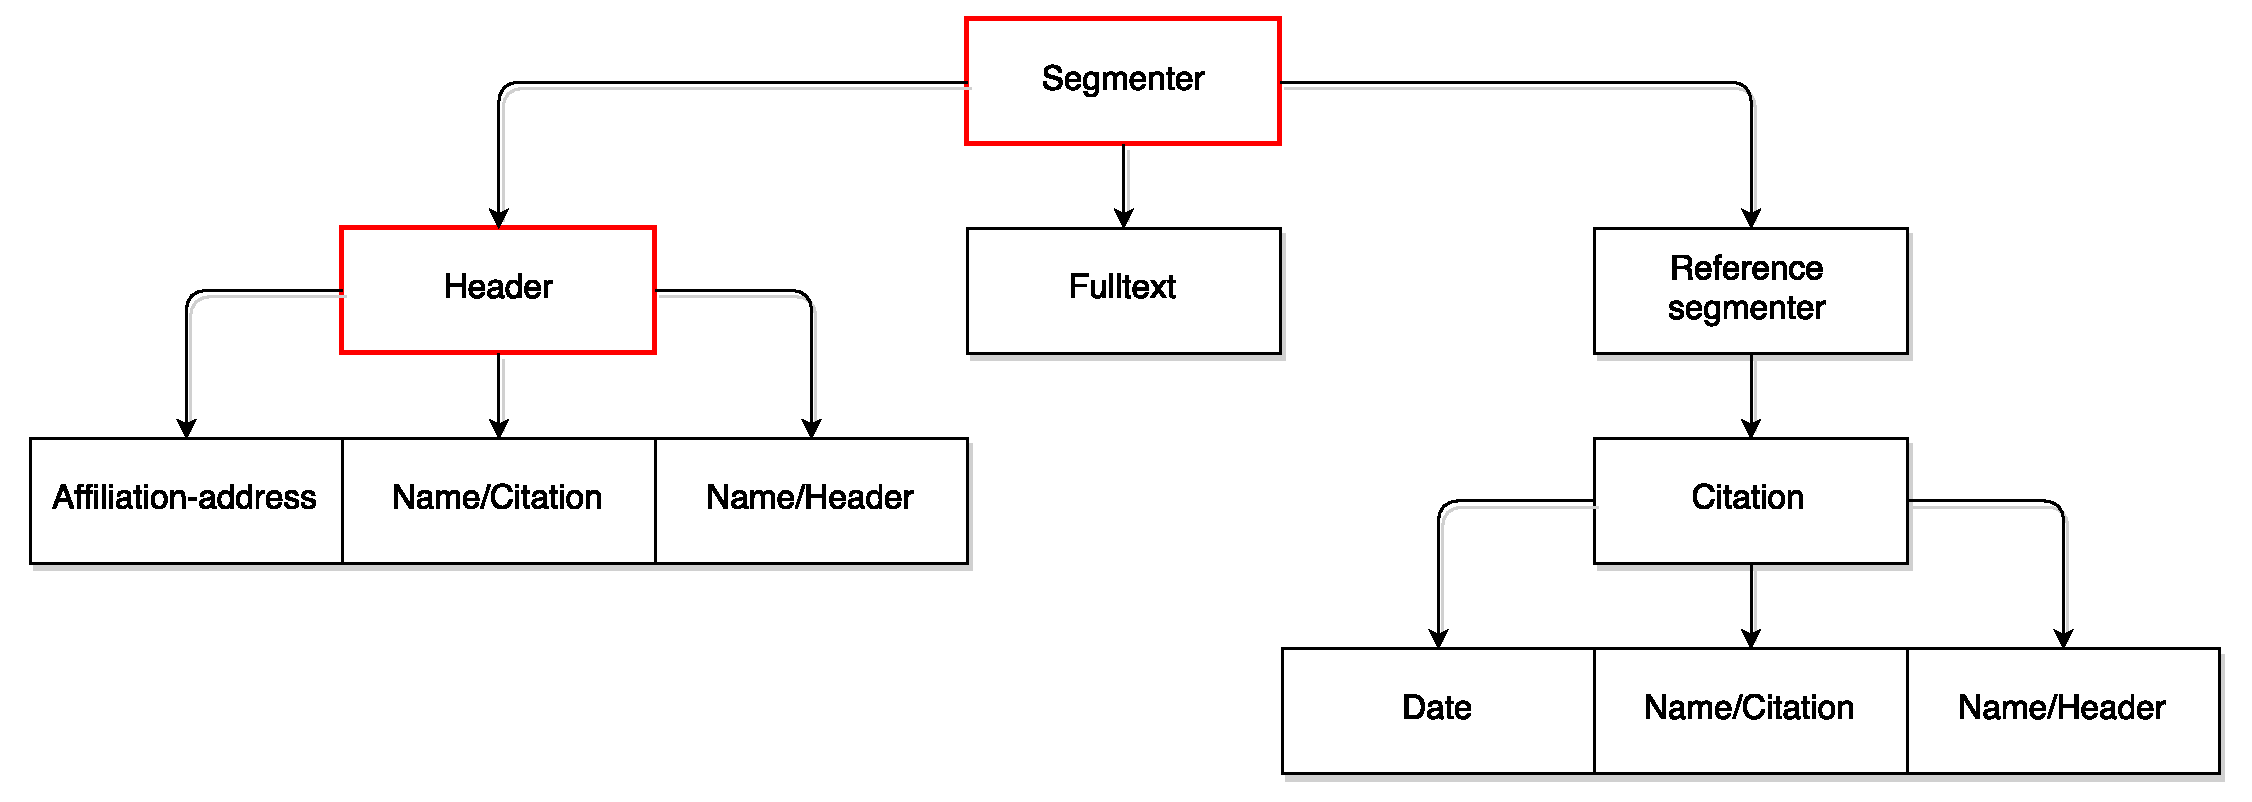
\includegraphics[width=\textwidth]{Figures/cascade.pdf}
\caption{The models of Grobid are organised into a cascade, where each part of a document is classified in increasingly greater detail.}
\label{fig:cascade}
\end{figure}

\subsection{Comparison with REFEXTRACT}

By way of a benchmarking evaluation for GROBID, we compare it with REFEXTRACT, the existing solution. As mentioned earlier, this existing tool is incomplete and greatly lacking in the . It is capable only of retrieving references\footnote{A comparatively easy task; GROBID's citation model usually performs at a significantly higher accuracy than, say, the header model.}, and the classification itself is quite basic. Since the modelling of reference fields differs between the two, a comparison is difficult to make. A comparison will at least be indicative, however, and we are able to make reasonable comparisons on the most important fields. The dataset for the comparison consists of 60 articles coming from the SCOAP$^3$ online repository\footnote{Scoap$^3$ (Sponsoring Open Consortium for Open Access Publishing in Particle Physics) is an open access digital library hosted at CERN, backed by an international partnership of research institutions.}.

Unlike REFEXTRACT, GROBID requires two separate models to classify the citations of a given article: the reference-segmenter and citation models\footnote{Strictly speaking, there is another model, (full) Segmentation, above the reference-segmenter, and so citation accuracy depends on this also. But because one focus of our work is to improve this model, we accept this omission.}. The former . Therefore, the accuracy of the citation model is ultimately subject to the accuracy of the refernence block inputs supplied to it. The citation model, unlike

\label{subsec:refextract}
\begin{table}[h]
\begin{center}
\begin{tabular}{|c|cccc|}
\hline
label		&accuracy	&precision	&recall		&f1 \\
\hline
<label>		&99.96		&100		&99.2		&99.6\\
<reference>		&99.96		&99.96		&100		&99.98\\
\hline
(micro average) & 99.96		&99.96		&99.96		&99.96	\\
(macro average) &	99.96 & 99.98	& 99.6 & 99.79	\\
\hline
\end{tabular}
\caption[Evaluation results for reference segmentation]{Evaluation results for reference segmentation}
\label{table:referencesegmenterresults}
\end{center}
\end{table}

\begin{table}[h]
\begin{center}
\begin{tabular}{|c|cccc|cccc|}
\hline
engine &  \multicolumn{4}{c}{GROBID} & \multicolumn{4}{c}{REFEXTRACT}\\
\hline
label & accuracy & precision & recall & f1 & acc. & prec. & rec. & f1\\
\hline
<author>	&	99.85	&	99.68	&	99.75	&	99.72 	& 98.33	&	100	&	92.22	&	95.95	\\
<title>	&	99.59	&	98.87	&	99.25	&	99.06 	& 94.89	&	100	&	71.75	&	83.55	\\
<journal>	&	98.84	&	88.87	&	93.98	&	91.35 	& 97.12	&	100	&	46.78	&	63.74	\\
<volume>&	99.95	&	99.07	&	98.15	&	98.6 		& 98.36	&	0	&	0		&	0	\\
<issue>	&	99.93	&	100		&	94.63	&	97.24	 & 98.87	&	0	&	0		&	0	\\
<pages>	&	99.75	&	93.51	&	99.45	&	96.39 	& 97.26	&	0	&	0		&	0	\\
<date>	&	98.39	&	57.39	&	98.31	&	72.47 	& 98.88	&	100	&	37.55	&	54.6	\\
<pubnum>&	98.71	&	100		&	12.96	&	22.95 	& 98.77	&	0	&	0		&	0	\\
<note>	&	99.4	 	&	43.75	&	35		&	38.89 	& 99.55	&	0	&	0		&	0	\\
<publisher>&	99.81	&	63.46	&	94.29	&	75.86 	& 99.73	&	0	&	0		&	0	\\
<location>&	99.81	&	86.32	&	91.11	&	88.65 	& 99.32	&	0	&	0		&	0	\\
<institution>&	99.78	&	25		&	25		&	25 		& 99.88	&	0	&	0		&	0	\\
<booktitle>&	98.7		&	55.56	&	41.67	&	47.62 	& 98.82	&	0	&	0		&	0	\\
<web>	&	99.64	&	51.85	&	100		&	68.29 	& 99.68	&	0	&	0		&	0	\\
<editor>	&	99.93	&	100		&46.67		&	63.64 	& 99.89	&	0	&	0		&	0	\\
<tech>	&	99.95	&	83.33	&	50		&	62.5 		& 99.92	&	0	&	0		&	0	\\
\hline
(micro average) & 99.5	&	93.63	&	94.77 	&	94.19 & 98.7	&	100	&	63.47 	&	77.65	\\
(macro average) & 99.5	&	77.92	&	73.76	&	71.76 & 98.7	&	25	&	15.52	&	18.62	\\
\hline
\end{tabular}
\caption[Evaluation results for citations]{Evaluation results for citations}
\label{table:citationcomparison}
\end{center}
\end{table}
